\chapter{Introduction} \index{Introduction@\emph{Introduction}}%

\section*{Preface}
\addcontentsline{toc}{section}{Preface}%

    Heart valves play a critical role of preventing back flow during cardiac operations. They are designed to withstand the demanding mechanical environment of the heart while maintaining optimal state for over 3 billion cycles. When they can no longer function properly due to fatigue, diseases or trauma, and surgical repair is not an option, surgical replacement using bioprosthetic heart valves is often the best choice. This introductory chapter focus on the current state of heart valve replacements and design, and methods for improving the durability of these devices. First, an overview of the structure and functions of heart valves is provided. Then the current state of heart valve repair and replacement is summarized, followed by the current state of bioprosthetic valve design and fabrication as well as they durability and limitations. Finally, the causes and mechanisms of bioprosthetic heart valve failure is discussed, and we outline the motivation, rationale and aims of this dissertation, on how constitutive modeling and simulations can be used to better understand bioprosthetic heart valve failure and facilitate the improvement of bioprosthetic heart valve design. 

\section{Introduction and Background}
\section{Introduction and Background}

    Cardiovascular diseases remain the leading cause of death (31.8\% of all deaths) in U.S., costing 320.1 billion each year \cite{mozaffarian_heart_2015}. One significant area that need improvements is heart valve replacement and repair procedures such as aortic valve repair using bioprosthetic heart valves (BHVs), where the mortality has not seen any major improvements since 1985 – the rate of survival after 10 years still remains only 29.7\%. Soft-tissue-derived exogenously cross-linked (EXL) biomaterials, which has only existed since the beginning of 1970s, is the dominant choice due to advantages in immunogenicity and flow dynamics over their mechanical counter parts \cite{starr_artificial_2007}. However, our understanding of these materials and of the mechanisms of their failure is still incomplete. As such, current design and development is very empirical in nature – depending on trial and error, extrapolation from accelerated wear test and long periods of clinical testing. The need for better BHV designs is further accelerated by the emergence of percutaneous devices such as the transcather aortic valve replacement (TAVR) \cite{bonow_accaha_2006}\cite{guidoin_marvel_2010}. TAVRs are an attractive alternative to open heart surgeries, especially for people at high surgical risk, as well as youths who may require multiple surgical replacements over their life-time. However, they are more often associated with peri-valvular regurgitation and is currently lacking in long-term data pertaining to their durability \cite{guidoin_marvel_2010}. Existing TAVR data suggest only 2-year mortality rate of 33.9\% \cite{kodali_two_2012} in general and 68\% for aortic valve stenosis \cite{makkar_transcatheter_2012}. Much of the existing challenges is associated with the necessary compact folded delivery system, which places additional constraints on their geometrical design and mechanical properties. It is clear that there is a strong need for a better understanding of the mechanism associated with their failure and frameworks for predicting the long-term failure of these devices.
        
    

    
    
    
    
    
    




\section{Structure and function of heart valves}
\subsection{Multi-scale structure of heart valves}

    To fully understand the functional properties of heart valves, multi-scale approaches are needed (Fig. \ref{fig:multiscalevalve}) \cite{salma_heart_2016}. This complex hierarchical structure is what lends to seamless heart valve performance under highly dynamic loading conditions. Heart valves have evolved to have multi-layered leaflet structures. The aortic valve, for example, consists of three histologically distinct layers, whereas the mitral valve has four (Fig. \ref{fig:valvelayers}). The fibrosa layer, which is located on the ventricular side of atrioventricular valves and the atrial side of semilunar valves, is composed of circumferentially aligned collagen fibers that provide the leaflets with the necessary tensile strength to open and transmit forces during coaptation while closed. The spongiosa layer is situated adjacent to the fibrosa and though it contains some collagen, its main constituents are the hydrophilic glycosaminoglycans and proteoglycans, which give the valve its compressive properties and allow it to absorb high forces during coaptation. The ventricularis and atrialis are the layers that are adjacent to blood flow in atrioventricular valvesand semilunar valves, respectively. These layers are rich in radially oriented elastin fibers and facilitate the closure movement by extending the valve leaflet as it opens and recoils when it closes. The annulus and chordae tendineae of the atrioventricular valves and the connection between the leaflets and the surrounding myocardium in the semilunar valves provide additional support. 


    Each layer contains varying amounts of collagen, glycosaminoglycan (GAG), and elastin \cite{carruthers_gene_2012}. The fibrosa layer, facing the outflow surface, consists primarily of a dense network of highly aligned type 1 collagen fibers and contributes to about 45\% of the valve thickness. The central spongiosa layer, approximately 30\% of the leaflet thickness is rich in glycosaminoglycans and water \cite{carruthers_gene_2012}. The ventricularis layer, the remaining 25\% of the leaflet faces the left ventricle inflow surface and is composed of elastin and disorganized collagen. Taken collectively, the three layers of the AV with their elastin, collagen and glycosaminoglycans constituents comprise the ECM of the valve. In addition to the biomechanical role the ECM plays in valve function, it provides a support structure for the underlying valve cell network. The ECM influences cell behavior by providing a source of ligands for cell surface receptors, which transfer mechanical strains experienced at the tissue level down to the cells and ultimately initiating intracellular signaling pathways \cite{wiltz_extracellular_2013}.


%-------------------	begin FIGURE 	-------------------%
\begin{figure}
\centering
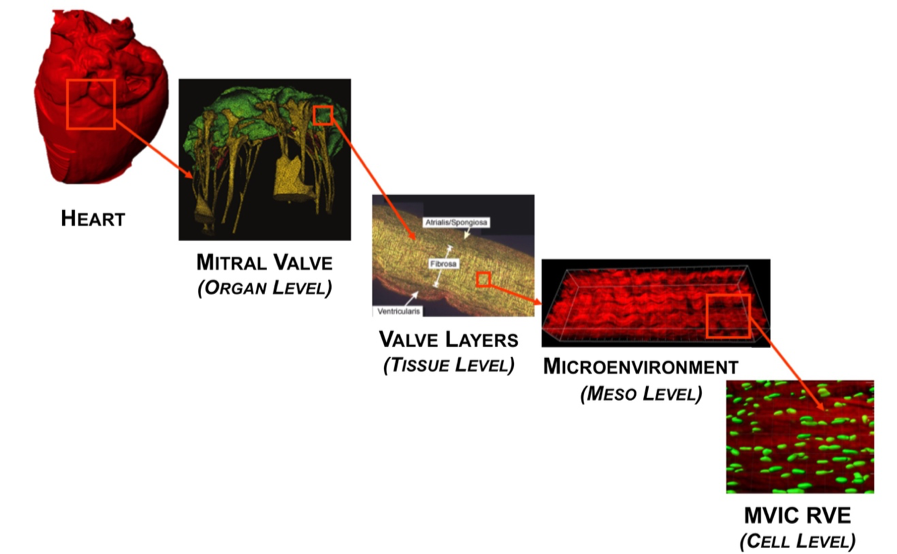
\includegraphics[width=\textwidth]{Images/chapter1/multiscalevalve.png}
\caption{The multiscale nature of heart valve biomechanics: a representation of the mitral valve at the organ-, tissue-, and cell-levels. At the tissue-level: a circumferentially oriented cross-section of the mitral valve anterior leaflet stained with Movat pentachrome, which colors collagen yellow, elastic fibers black, and hydrated PGs and GAGs blue. At the cell-level: a transmission electron micrograph of a mitral VIC from the fibrosa layer. \cite{salma_heart_2016}}
\label{fig:multiscalevalve}
\end{figure}
%-------------------	 end FIGURE 	-------------------%


%-------------------	begin FIGURE 	-------------------%
\begin{figure}
\centering
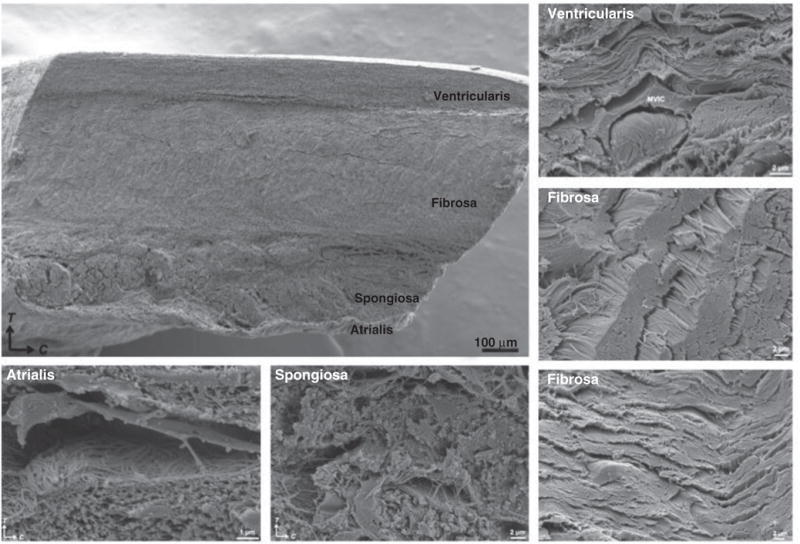
\includegraphics[width=\textwidth]{Images/chapter1/valvelayers.jpg}
\caption{Scanning electron micrograph of the multilayered microenvironment of the MV anterior leaflet. Individual micrographs of each layer are also presented: elastin-rich ventricularis and atrialis, highly collagenous fibrosa, and proteoglycan-rich spongiosa. The collagen fibrils and elastic fibers closely surround the interstitial cells and highlight the long cellular extensions. In the fibrosa, collagen fibrils are aligned in the circumferential direction of the leaflet, which is responsible for the observed anisotropy in leaflet mechanical behavior. (T: transmural, C: circumferential). \cite{salma_heart_2016}}
\label{fig:valvelayers}
\end{figure}
%-------------------	 end FIGURE 	-------------------%




\subsection{Biomechanical function of heart valves}

It has been demonstrated that the individual layers of the aortic valve are not only vastly different in their structure, but also in their mechanical behavior. Two key studies have investigated individual layer behavior of the AV leaflet. Vesely et al. observed the extensibility of intact tissue under uni-axial tension to be significantly different from the individual layer responses [71]. Stella et al. also observed measurably different behaviors under bi-axial loading of separated layers, and reported the intact tissue response to be intermediate to the separated responses [72]. Due to these consistently observed differences in layer behavior, examining the leaflet in an intact state is far more physiologically relevant. 

\section{Valvular diseases and prevalence}
\section{Valvular diseases and prevalence}

    Cardiovascular diseases are the number one killer in the United States and around the world. Heart valve treatment is a common cardiovascular surgical procedure with over 100,800 done annually in the U.S. alone \cite{mozaffarian_heart_2016} and 275,000 to 370,000 in developed nations \cite{manji_future_2012}. Calcification is the primary cause of AV failure and currently there exists no proven therapy for halting this progression. Calcified aortic valve disease is a slow, progressive, multi-factorial disorder that is more common with age, without being an inevitable consequence of aging \cite{towler_molecular_2013,freeman_management_2002,freeman_spectrum_2005,kurtz_aortic_2010,beckmann_insights_2010}. The disease is characterized by a thickening and calcification of the leaflets and is diagnosed in two stages: aortic sclerosis and aortic stenosis. aortic sclerosis, present in more than 25\% of patients over the age of 65 \cite{obrien_pathogenesis_2006}, represents the early onset of calcified aortic valve disease absent of physical obstruction to the left ventricular outflow. Aortic stenosis exists in 2-5\% of the elderly population \cite{obrien_pathogenesis_2006} is characterized by late stage obstruction and associated with impaired leaflet motion, valve tissue adaptation, and resistance to blood flow \cite{poggio_noggin_2013,grau_analysis_2012,gharacholou_aortic_2011,pflederer_aortic_2010} . Although aortic sclerosis causes significant thickening of the AV leaflets, there is little to no change in the mechanical properties of the valve, making the disease relatively asymptomatic. Recent statistics have shown that within 10 years of their initial diagnosis, 10\% of aortic sclerotic patients reach a state of severe calcified aortic valve disease that requires immediate AV replacement once symptoms emerge \cite{gharacholou_aortic_2011}. 
    
    
    Aortic stenosis has been identified as the end-stage of calcified aortic valve disease that progresses from the microscopic early changes of aortic sclerosis to, in a subset of patients, asymptomatic and then symptomatic Aortic stenosis \cite{kurtz_aortic_2010,otto_calcific_2010,aikawa_look_2012}. Once aortic sclerosis is detected, there is an increased risk of cardiovascular events. In early Aortic stenosis, when mild symptoms begin to present, survival rates deviate much more than expected and decline dramatically with the onset of severe symptomatic Aortic stenosis. Over the last decade, several clinical trials, mostly extensions of atherosclerosis-related studies, have been performed to halt the progression of calcified aortic valve disease with randomized studies showing substantial equivalence between treatments and placebo \cite{parolari_do_2011,moura_rosuvastatin_2007,cowell_randomized_2005,benton_statins_2009,rossebo_intensive_2008}. However, there are currently no pharmacological therapies available to treat calcified aortic valve disease symptomatic patients that are considered superior to full valve replacement surgery. 




\section{Surgical repair and replacement}


\section{Heart valve prosthesis}

\subsection{Brief history of the development of heart valve replacements}

\subsection{Advantages of tissue-engineered valves}

\subsection{Fabrication of bioprosthetic heart valves}

\subsection{Current and future technology on bioprosthetic heart valves}




\section{Bioprosthetic heart valve durability and limitations}

\subsection{Bioprosthetic heart valve life-span}

\subsection{Limitations in bioprosthetic heart valve design and fabrication}


\section{Causes of bioprosthetic heart valve failure}

\subsection{Biological and mechanical aspects of fatigue}

\subsection{Brief summary on the role of calcification}

\subsection{Mechanical fatigue and failure}

\section{Motivation, rationale, and specific aims}

    Soft-tissue-derived exogenously cross-linked (EXL) biomaterials continue to play an important role in surgical repair and medical devices. This is especially true for bioprosthetic heart valves (BHV), by having advantages in immunogenic and mechanical behaviors [1]. Despite ongoing research, our understanding of these materials and of the mechanisms leading to their failure remains at an empirical level. The need for advancements in predicting the material behavior is further underscored by the development of percutaneously-delivered BHV devices. While these devices reduce surgical risk, they also present additional challenges for the design of the BHVs due to limitations in thickness, and folding and compression during delivery. A significant challenge prohibiting accurate and predictive simulations of BHVs are a lack of understanding of the effect of exogenous cross-linkers, such as glutaraldehyde (GLUT), and an associated predictive material model in response to cyclic loading. GLUT EXLs form polymeric chains through the cross-linking process which more tightly bond the collagen fibers to the non-fibrous matrix, increasing the non-fibrous matrix stiffness and fiber-fiber interactions. However, GLUT EXLs also undergo Schiff-base reactions that are hypothesized to lead to scission-healing behaviors that result in the permanent set (PS) phenomena. PS continuously changes in the reference geometry of the BHV and can induce extra-physiological stress concentrations in the BHV leaflets. Microstructural-based constitutive models for tissues and their use in valve-level simulations can lead to insights into the underlying mechanisms and more accurate prediction of their long-term performance. Thus, we seek to develop a framework for modeling and simulating biologically-derived EXL soft collagenous tissues for BHV, accounting for the effects of EXL, PS, and collagen fiber-level damage, taking the following approach:


    \subsubsection*{Specific Aim 1: Establish and validate a generalized nonlinear hyperelastic meso-scale structural constitutive model (MSSCM) for native collagenous soft tissues.} As a first step towards modeling EXL biomaterials, we will take a generalized meso-scale (at the level of the constituent fibers) structural modeling approach to accurately model the mechanical response of soft tissues. Firstly, we will develop an improved analytical method for processing extant mechanical data under generalized 2D deformations, to more accurately characterize the tissue. Next, after posing the model form, we will extensively validate critical assumptions such as affine fiber deformation, mechanical response of the constituent fibers, and direct integration of physical measurements of the fiber microstructure. The validation will be done through extensive mechanical characterization through different testing methods and microstructural characterization at the 1) micro-scale (fibril) and 2) meso-scale using optical techniques such as multiphoton microscopy and x-ray scattering. The two tissues we will examine for application and validation of the model are the ovine pulmonary artery and the porcine mitral valve leaflets, which offer a diverse selection structural composition to span applicable realms.
    
    \addcontentsline{toc}{subsubsection}{Specific Aim 1: Establish and validate a generalized nonlinear hyperelastic meso-scale structural constitutive model for native collagenous soft tissues.}%


    \subsubsection*{Specific Aim 2: Extend the MSSCM to account for of the presence of EXLs and subsequent response to continuous cyclic loading.} Using GLUT treated bovine pericardium, we aim to separately model the mechanical response of the collagen fibers, matrix, and fiber-fiber interactions due to cross-linking. For this, we will develop a method to map the collagen fiber architecture characterized from the native state to the EXL state. Next, we will develop a PS model based on a constantly evolving referential configuration that occurs due to scission-healing when the tissue is held in an extended state. We will validate the model for orientation and strain level dependence. The model will be tested and validated using constant cyclic strain, as well as stress control experimental data. Finally, we will extend the model for collagen fiber-level damage that may occur during cyclic loading. 
    
    \addcontentsline{toc}{subsubsection}{Specific Aim 2: Extend the meso-scale structural constitutive model to account for of the presence of EXLs and subsequent response to continuous cyclic loading.}%
    
    
    \subsubsection*{Specific Aim 3: Application to organ/device level}. In this final aim, we will develop a full 3D finite element implementation utilizing the open source FEniCS framework for greater modularity and extensibility. The model will utilize real BHV geometries and fiber microstructure mapped from experimental measurements, and will be validated by simulating of the PS experiments from SA 2. We will further perform organ-level study of PS and collagen fiber-level damage using accelerated wear testing of specialized ovine mitral transcutaneous BHVs. We will use an inverse modeling approach with micro-CT measurements [2] to quantify changes in mechanical behaviors. The validated model and rate constants will then be used to parametrically examine the changes in BHV geometry and stress distribution overtime, where change in resting and loaded geometry of the valve as well as the development of stress concentrations are the early indicators of BHV failure. We will also explore initial geometries and material properties which may minimize the risks of these effects. With this, we aim to develop a better understanding of the underlying process that occurs during long-term cyclic loading using our constitutive modeling approach and device level applications, and translate the insights gained to improving BHV design and durability. 

    \addcontentsline{toc}{subsubsection}{Specific Aim 3: Application to organ/device level}%

\bibliographystyle{plainnat}
\bibliography{phd}



